\documentclass[a4paper, 10pt]{article}

\usepackage{amsmath}
\usepackage{siunitx}
\usepackage{graphicx}
\usepackage[T1]{fontenc}
\usepackage[utf8]{inputenc}
\usepackage[english]{babel}
\usepackage[sc]{mathpazo}
\usepackage{color}

% Various spacing parameters
\usepackage{microtype}
\usepackage[margin=3.5cm]{geometry}
\linespread{1}
\parindent 0pt
\parskip 4pt

% Helping functions
\newcommand{\pdiff}[2]{\frac{\partial #1}{\partial #2}} % Partial derivative

% Spacing inside description environment
\usepackage{enumitem}
\setlist[description]{style=multiline,leftmargin=.8cm,parsep=4pt}

\title{Fluid Dynamics + Turbulence (fall 2017)\\Homework Problems II + voluntary Exercises}
\author{}
\date{}

%----------------------------------------------------------------------------------------

\begin{document}
\maketitle

\large{
\textbf{Posted:}
\today

\bigskip
\textbf{Deadline:}
September 11 (Tuesday) at 08:30 am (on Blackboard).
}

\bigskip

\section*{Homework problem 1.1: Why does an Airbus A380 fly?}
\begin{description}
\item[(a)]
Use the Navier-Stokes equation in the static limit $\vec{u}=0$, the gravitational force $\vec{f}_\mathrm{ext} = -\rho g \vec{e}_z$,  and the equation of state $p/p_0=\rho/\rho_0$ to derive the barometric height formula
\begin{equation*}
    \frac{p(z)}{p_0} = \frac{\rho(z)}{\rho_0} = \exp \left(-\frac{g\rho_0 z}{p_0}\right),
\end{equation*}
where $z$ is the height above ground, $p_0=p(z=0)=\SI{1.01e5}{\frac{kg}{m\, sec^2}}$ is the air pressure at ground, $\rho_0=\rho(z=0)=\SI{1.20}{kg/m^3}$ is the air density at ground, and $g=\SI{9.81}{m/sec^2}$ is the acceleration of gravity. How much is the air density reduced at the height $z=\SI{10}{km}$ above ground?

\item[(b)]
An Airbus A380 is typically cruising with the velocity $u=\SI{945}{km/h}$ at a height \SI{10}{km} above ground. The lift force acting on the air wings is balancing the weight force. Use Bernoulli's equation to make a rough estimate of the velocity difference above and below the air wings. All you need are the results from (a), the wing area $A_{wing} = \SI{846}{m^2}$ and the weight $m \approx \SI{500}{t}$ of the A380.
\end{description}

\newpage
\section*{Homework problem 2.2: Surface bump or dip in a shallow river flow?} 
Consider an ideal two-dimensional shallow river flow over a small bump at the river bed; see sketch.
\begin{figure}[h!]
	\centering
	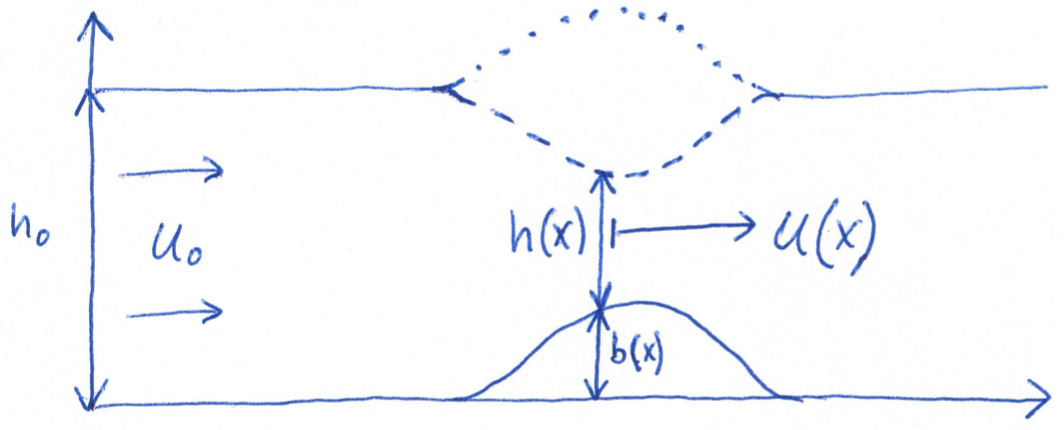
\includegraphics[width=.7\textwidth]{bump.png}
\end{figure}

{\bf (a)} Explain the two conservation laws: 
\begin{eqnarray}
	u_0 h_0 &=& u(x) h(x) \; , \\
	\frac{u_0^2}{2} + g h_0 &=& \frac{u^2(x)}{2} + g \left( b(x) + h(x) \right) \; .
\end{eqnarray}
{\bf (b)} Equations (1) and (2) are two equations for the two unknown functions $h(x)$ and $u(x)$. Eliminate $u(x)$ and derive an equation only for $h(x)$. Show that this equation is consistently solved by $h(x)=h_0$ when $b(x)=0$. In order to solve the equation also for $b(x)>0$, assume the bump $b(x)\ll h_0$ and the change of river surface height $\Delta h(x) = h(x)-h_0\ll h_0$ to be small. Derive the solution
\begin{equation}
	\Delta h(x) = \frac{b(x)}{\left(\frac{u_0^2}{gh_0}-1\right)}
\end{equation}
by keeping first-order terms in small $b(x)/h_0$ and $\Delta h(x)/h_0$ in a consistent way. \newline

{\bf (c)} Use equation (3) in the two limits $u_0^2\ll gh_0$ and $u_ 0^2 \gg g h_0$ to explain when a surface bump or dip occurs. \newline

{\bf (d)} What is the catch with equation (3) when $u_0^2\approx gh_0$? \newline

{\bf (e)} Use the numbers $b_\mathrm{max}=\SI{0.1}{m}$, $h_0=\SI{1}{m}$, $g=\SI{9.81}{m/s^2}$ to calculate the extremum of $\Delta h(x)$ for $u_0=\SI{1}{m/s}$ and $u_0=\SI{10}{m/s}$.
\newpage


\section*{Exercise 2.1}
The friction force in the Navier-Stokes equation
\begin{equation}
    \rho \left(\pdiff{\vec{u}}{t} + \left(\vec{u}\cdot\vec{\nabla}\right)\vec{u}\right) =
    \vec{f}_{\mathrm{ext}} - \vec{\nabla}p + \mu \left(\vec{\nabla}\cdot\vec{\nabla}\right)\vec{u} +
    \left(\mu_v + \frac{\mu}{3}\right)\vec{\nabla}\left(\vec{\nabla}\cdot\vec{u}\right)
\end{equation}
contains the term
\begin{equation}
    \pdiff{^2u_y}{x\partial y}
\end{equation}
in x-direction. Why does this term represent a force pointing in the x-direction?


\section*{Exercise 2.2}
An infinitesimal closed line integral can be approximated as
\begin{align}
    \begin{split}
        \oint\vec{v}(x,y)\cdot d\vec{s} &\approx v_x\left(x,y+\frac{\Delta y}{2}\right)\Delta x \\
        &\hspace{5mm}+ v_y \left(x+\frac{\Delta x}{2}, \Delta y\right)(-\Delta y)\\
        &\hspace{5mm}+ v_x \left(x, y-\frac{\Delta y}{2}\right)(-\Delta x)\\
        &\hspace{5mm}+ v_y \left(x-\frac{\Delta x}{2}, y\right) \Delta y.
    \end{split}
\end{align}
Use a Taylor series expansion and show that
\begin{equation}
    \oint \vec{v}\cdot d\vec{s} = - \left(\vec{\nabla}\times\vec{v}\right)\cdot\vec{e}_z \Delta x \Delta y
\end{equation}
Given this result, illustrate what the irrotational flow condition $\vec{\nabla}\times\vec{v}=0$ means.

\section*{Exercise 2.3}
Consider the following two-dimensional velocity field:
\begin{align}
	u_x &= u_0\\
	u_y &= \kappa x^2
\end{align}

\begin{description}
	\item[(a)]
	Sketch the velocity vector at selected positions along the $x$-axis.
	
	\item[(b)]
	Calculate the divergence $\vec{\nabla}\cdot\vec{u}$ and curl $\vec{\nabla}\times \vec{u}$ of the velocity field.
	
	\item[(c)]
	Use the differential equations
	\begin{equation}
		\frac{\mathrm{d}x}{\mathrm{d}t} = u_x, \quad \frac{\mathrm{d}y}{\mathrm{d}t} = u_y
	\end{equation}
	to show that if a particle is in position $(x_0,\, y_0)$ at time $t_0$, then at time $t$ its position is given by
	\begin{align}
		x(t) &= x_0 + u_0(t-t_0)\\
		y(t) &= y_0 + \frac{\kappa}{3u_0}\left[x(t)^3 - x_0^3\right].
	\end{align}
	
	\item[(d)]
	Sketch some particle trajectories (path lines) with $t_0=x_0=0$.
\end{description}

\section*{Exercise 2.4}
When we derived the Bernoulli equation
\begin{equation}
    \frac{\rho_0}{2}\vec{v}^2+p=\mathrm{constant},
\end{equation}
we stumbled over the relation
\begin{equation}
    \vec{\nabla}\left(\frac{\rho_0}{2}\vec{v}^2+p\right) = \rho_0\vec{v}\times\left(\vec{\nabla}\times\vec{v}\right),
\end{equation}
where we simply evoked the irrotational flow condition to put the right-hand side to zero. Now we want to be more careful.

\begin{description}
    \item[(a)]
        Show that when we multiply (scalar product) the right-hand side with a segment $d\vec{s}$ of a streamline, that
        \begin{equation}
            d\vec{s}\cdot\left[\vec{v}\times\left(\vec{\nabla}\times\vec{v}\right)\right]=0.
        \end{equation}

    \item[(b)]
        Show that the integration of the left-hand side,
        \begin{equation}
            \int\vec{\nabla}\left(\frac{\rho_0}{2}\vec{v}^2+p\right)\cdot d\vec{s} = 0,
        \end{equation}
        along a streamline, leads to
        \begin{equation}
            \frac{\rho_0}{2}\vec{v}^2+p=\mathrm{constant}=c
        \end{equation}
        along the streamline.

    \item[(c)]
        What can you say about the constant $c$ for different stream lines?
\end{description}


\end{document}